% Basics
\documentclass{article}
\usepackage[utf8]{inputenc}

% Graphics
\usepackage{graphicx}
\usepackage{titlepic}
\graphicspath{ {./images/} }

% Margins
\usepackage{geometry}
\geometry{ a4paper,
           total={170mm,257mm},
           left=20mm,
           top=20mm }
           
% Diagrams
\usepackage{tikz}
\usetikzlibrary{er,positioning}
\usepackage{pgf-umlsd}
\usepgflibrary{arrows} 

% Pseudo code
\usepackage{algorithm}
\usepackage{algorithmic}

% Maths
\usepackage{amssymb}
\usepackage{amsmath}
\usepackage{commath}

% To display URL in biblio
\usepackage{hyperref}

% Cover page
\title{IMU Data Recovery, Processing and Display}
\author{ Decho Surangsrirat \\
         NECTEC, Thailand 
         \and 
         Vincent Maire\\
         INSA Toulouse, France }
\date{July 2018}

\begin{document}
\maketitle

%%%%%%%%%% Begin %%%%%%%%%%%

\section{Abstract}

This project aims to develop a system able to determine its own relative orientation in space. It uses an Inertial Motion Unit (IMU): MPU9250. This IC is a 10 degrees of freedom sensor as it provides a 3D acceleration vector, an angular speed in both 3 coordinates, the intensity of the Earth Magnetic Field for each 3 axis, and the sensor's temperature. 

The system consequently designed must be generic enough to be used as assistant for several and various medical tasks. However, to prove the accuracy and robustness of the system, it will be tested as an assistant for surgical screw implantation to improve the free hand technique, using the Jost et al paper \cite{jost} as reference. Thus, the software used in the present project has been rearranged to match with such a purpose. 

This report will first describe the hardware used and its implementation. Then, it will cover the structure of the developed software and will detail the chosen solutions. Finally, it will explore the possible improvements that can be made and sum up this project.


\section{Hardware architecture}

As described in the figure \ref{fig:basic_architecture}, the system is divided into 3 main hardware components:
\begin{itemize}
    \item The MPU9250 board which is the 10 DOF IMU
    \item An Arduino Nano, which communicates with the MPU9250 through an I2C protocol and recover the raw data
    \item A C\# software, developed under Visual Studio, and yields the data from the Arduino to filter it, convert it into a quaternion representation and display the results to an user-friendly interface 
\end{itemize} 

\begin{figure}[ht]
    \centering
    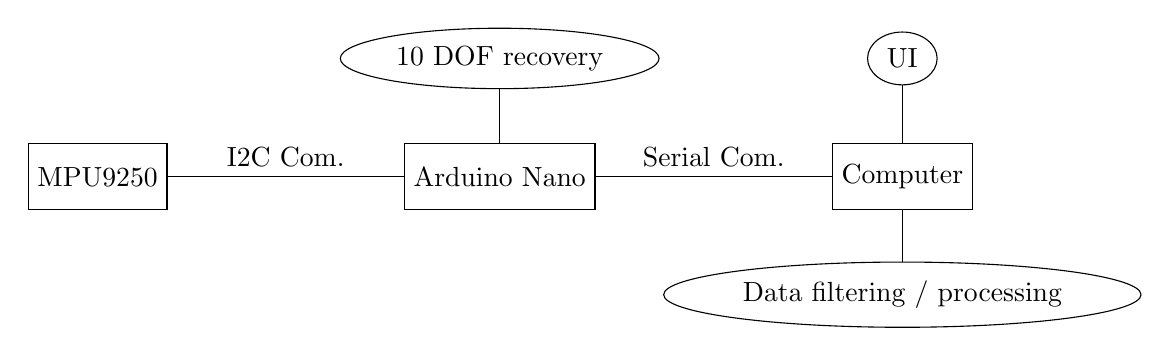
\begin{tikzpicture}[auto,node distance=3cm]
      \node[entity] (mpu) {MPU9250};
      \node[entity] (ard) [right = of mpu] {Arduino Nano}
      child [grow=up] {node[attribute] {10 DOF recovery}};
      \node[entity] (com) [right = of ard] {Computer}
      child [grow=up] {node[attribute] {UI}}
      child [grow=down] {node[attribute] {Data filtering / processing}};
      \path (mpu) edge node {I2C Com.} (ard);
      \path (ard) edge node {Serial Com.} (com);
    \end{tikzpicture}
    \caption{Basic architecture of the developed system}
    \label{fig:basic_architecture}
\end{figure}

\section{Arduino configuration}

Only 4 wires are required to recover the data from the MPU9250:
\begin{itemize}
    \item POWER: 3.3V/GND
    \item I2C Com.: SCL/SDA
\end{itemize}

The software downloaded on the Arduino \cite{fabo_library} is open source, shared by FaBo and distributed under Apache license 2.0 (non-restrictive).

\vspace{\baselineskip}

The Arduino only perform once the accelerometer and gyroscope calibration. However, the magnetometer data are still soft and hard iron biased (among others). Then, the raw values $\{ax, ay, az, gx, gy, gz, mx, my, mz, temp\}$ are transmitted through a high speed serial communication to the filtering and processing software. 

\section{Software's structure}

Written in C\#, developed with Visual Studio and implemented on a computer (Windows OS), this software has the capability to take 9 DOF raw data, process it into an understandable representation and display it to the user. An overview screenshot is displayed n figure \ref{fig:overview_screenshot}. 

\begin{figure}[ht]
  \centering
  \includegraphics[width=\textwidth]{images/overview_screenshot.png}
  \caption{Software overview screenshot}
  \label{fig:overview_screenshot}
\end{figure}

Basically, the program is made of 3 threads described in the pseudo sequence diagram in figure \ref{fig:seq_diagram}:
\begin{itemize}
    \item The serial thread that is triggered on data received. It parses the data from the serial and calibrate the received magnetometer values on-the-fly. 
    \item The filter thread that implement a Mahony filter. It is triggered on a timer interrupt with a period of 2ms. It output quaternions and Euler angles from the raw data.
    \item The display thread is also triggered on a timer with a period of 20ms. It refreshes the display of the Euler angles and the 3D view.
    
\end{itemize}

\begin{figure}[ht]
  \centering
  \begin{sequencediagram}
    \newthread{arduino_thread}{Arduino}
    \tikzstyle{inststyle}+=[below right=-0.85cm and 3cm of arduino_thread]
    \newthread{serial_thread}{Serial}
    \tikzstyle{inststyle}+=[below right=-0.85cm and 3cm of serial_thread]
    \newthread{filter_thread}{Filter}
    \tikzstyle{inststyle}+=[below right=-0.85cm and 3cm of filter_thread]
    \newthread{display_thread}{Display}    
    \begin{sdblock}{Loop}{On data read}
        \begin{messcall}{arduino_thread}{raw\_datas()}{serial_thread}
            \begin{callself}{serial_thread}{mag\_calibration()}{}
            \end{callself}
        \end{messcall}
    \end{sdblock}
    \begin{sdblock}{Loop}{$T=0.002s$}
        \begin{messcall}{serial_thread}{read\_calibrated\_datas()}{filter_thread}
            \begin{callself}{filter_thread}{mahony\_filter()}{}
            \end{callself}
        \end{messcall}
    \end{sdblock}
    \begin{sdblock}{Loop}{$T=0.010s$}
        \begin{messcall}{filter_thread}{read\_quaternions()}{display_thread}
            \begin{callself}{display_thread}{display\_UI()}{}
            \end{callself}
        \end{messcall}
    \end{sdblock}
  \end{sequencediagram}
  \caption{Sequence diagram}
  \label{fig:seq_diagram}
\end{figure}


\section{Magnetometer calibration} \label{sect_mag_cal}

Some corrections need to be done on the recovered magnetometer data. This section describes why this need to be calibrated and how we made it.

\subsection{Origin of the magnetometer biases}

Contrary to the gravity, the Earth magnetic field is not homogeneous everywhere on the planet. Thus, the magnetometer cannot use it as its reference to self calibrate. Moreover, the surrounding magnetic noise add some more uncertainty to the measurement. 

\subsection{Proposed solution}

A proposed solution described in the Renaudin et al paper \cite{renaudin} is to complete a full rotation of the IMU for each axis and to keep the minimum and maximum measured values. This solution has been implemented following the algorithm \ref{alg:cal_algo}. It loops for each data measurement, which means that the calibration is performed on-the-fly. The more the user rotates the IMU, the better. However, this process partially solve only soft and hard iron distortion.

\begin{algorithm}[H]
    \caption{Pseudo code for magnetometer calibration}
    \label{alg:cal_algo}
    \begin{algorithmic}[1]
        \STATE $min, max \in \mathbb{R}^3$
        \STATE $min \leftarrow \{+\infty, +\infty, +\infty\}$
        \STATE $max \leftarrow \{-\infty, -\infty, -\infty\}$
        \WHILE{$ True $}
            \IF{$ is\_raw\_data\_received $}
                \STATE $ mag \leftarrow read\_magnetometer() $
                \FOR{$ i \leftarrow 1;\ i < 3;\ i++ $}
                    \IF{$ mag[i] > max[i] $}
                        \STATE $ max[i] \leftarrow mag[i] $
                    \ELSIF{$ mag[i] < min[i] $}
                        \STATE $ min[i] \leftarrow mag[i] $
                    \ENDIF
                    \STATE $offset \leftarrow \frac{max[i]+min[i]}{2} $
                    \STATE $ calibrated\_mag[i] \leftarrow \frac{mag[i]-offset}{max[i]-min[i]} $
                \ENDFOR
            \ENDIF
        \ENDWHILE
    \end{algorithmic}
\end{algorithm}

\vspace{0mm}

\subsection{Results}

This solution has been tested and seems to be powerful enough for our specific application. The figure \ref{fig:cal_plots} shows the difference between the raw magnetometer measurements and the calibrated ones. We notice that the calibrated measurements are quite well circularized and normalized as they lie inside the black circle in the 2D plot. In the 3D plot, we want the measurement to fit in the black sphere.

\begin{figure}[H]
    \centering
    \includegraphics[height=10cm]{images/calibration_plot.png}
    \caption[Comparison between raw and calibrated data]
    {Comparison between raw data in \textcolor{red}{red} and calibrated data in \textcolor{blue}{blue}. (a), (b) and (c) are 2D views of the magnetic field intensity of each $x, y, z$ axis depending on another axis. (d) is a 3D plot of the magnetic field intensity depending on each axis.}
    \label{fig:cal_plots}
\end{figure}

However, this solution is the simplest to implement and is far to be perfect as it cannot compensate some of the sensor biases like sensor non-orthogonality. As the system is intended to be used in such places like hospitals, which contain many magnetic disturbances due to the heavy equipment and medical machines, finding a powerful calibration process should become an important feature to implement. Many research papers are dedicated to 3 axis magnetometer calibration. Vasconcelos et al propone in their study \cite{vasconcelos} a more powerful calibration using a geometrical approach, without needing the attitude of the IMU. Another research from Kok et al \cite{kok} uses the gyroscope and accelerometer to perform a magnetometer calibration.


\section{Orientation processing}

This section describes the computation steps required in order to get the IMU's orientation from the sensor's data.

\subsection{Mahony filter}

The system uses an open source implementation of a Mahony filter \cite{ximu_library}, a non-linear complementary filter, based on the work of Mahony et al \cite{mahony_filter}. It output the orientation in quaternion form. It is updated every $T = 5ms$ with a proportional gain $Kp = 15$ and integral gain $Ki = 0$.

\vspace{\baselineskip}

Watching closely to the MPU9250's datasheet, we notice that the orientation of the axes of sensitivity of the compass and the accelerometer are different. Thus, the order of the parameters fed to the filter have to be chosen carefully. In our case and in this order: $(g_x,\ g_y,\ g_z,\ a_x,\ a_y,\ a_z,\ m_y,\ m_x,\ -m_z)$.

\subsection{Using the quaternions}

\subsubsection{Quaternion rotation} \label{sub_sub_sect_quat_rot}

Quaternions are a powerful representation of the attitude as, among other advantages, require less computation to perform operations on them than Euler angles.

\vspace{\baselineskip}

\noindent
Let $v = (v_{1}, v_{2}, v_{3})$ be the 3D vector we want to rotate from the quaternion $q = (q_{1}, q_{2}, q_{3}, q_{4})$.

$$ v_{R} = 
\begin{bmatrix}
    1-2q_{2}^{2}-2q_{3}^{2}     &  2(q_{1}q_{2} + q_{0}q_{3})  &  2(q_{1}q_{3} - q_{0}q_{2}) \\
    2(q_{1}q_{2} - q_{0}q_{3})  &  1-2q_{1}^{2}-2q_{3}^{2}     &  2(q_{2}q_{3} - q_{0}q_{1}) \\
    2(q_{1}q_{3} + q_{0}q_{2})  &  2(q_{2}q_{3} - q_{0}q_{1})  &  1-2q_{1}^{2}-2q_{2}^{2}   
\end{bmatrix}
\begin{bmatrix}
    v_{1} \\
    v_{2} \\
    v_{3}   
\end{bmatrix}
$$

\vspace{\baselineskip}

In the same way, we can rotate a quaternion from another quaternion representation by multiplying them together.


\subsubsection{Quaternion to Euler representation}

Contrary to the Euler angles, quaternions lie into a 4 dimensional space, which make this representation gimbal lock issue free. However, it might be useful to display the Euler angles to the user are they are more understandable and readable. 

\vspace{\baselineskip}

Working with the proper Euler angles (not the Tait-Bryan ones), we should use the angles $[\Phi\ \Theta\ \Psi]$ but for more convenience, let's use in the same order
$[yaw\ pitch\ roll]$:


$$
\begin{bmatrix}
yaw \\
pitch \\
roll
\end{bmatrix} 
=
\begin{bmatrix}
atan2(2(q_0 q_1 + q_2 q_3),1 - 2(q_1^2 + q_2^2)) \\
asin(2(q_0 q_2 - q_3 q_1)) \\
atan2(2(q_0 q_3 + q_1 q_2),1 - 2(q_2^2 + q_3^2))
\end{bmatrix} 
$$

\section{Software features and usage}

This section explores the software features and presents an user-oriented how-to-use description.

\subsection{Features and their implementation}

\subsubsection{"Serial communication" box}

Contains a drop-down list to choose the serial port COM, a connect and disconnect button, and a refresh button that scans the available COM ports.

\subsubsection{"Configuration" box} \label{sub_sub_sect_config_box}

It contains a "Set origin button" which defines the current orientation as the new local frame following this process:

\vspace{\baselineskip}

\noindent
Let $q$ be the current measured quaternion from the Mahony filter, and $\Tilde{q}$ the new quaternion in the new reference frame. This new reference frame is saved when the user clicks "Set origin" by setting $q_0 = q$. Then, 
$$  
\Tilde{q} = q.q_0^{-1}
$$

\vspace{\baselineskip}

The second button in this box is "Reset calibration" and it used to reset the magnetometer's calibration. By clicking it, the user resets the algorithm \ref{alg:cal_algo} (breaks the loop and starts again at the first line). This button is essential as the current way to calibrate the magnetometer is performed on-the-fly and if a too strong magnetic disturbances is measured once, the calibrated measurements will become biased. 

\subsubsection{"Display" box and picture box}

The "Display" box manages what should be displayed in the picture box. 

\vspace{\baselineskip}

The picture box displays a cuboid and a compass in a 3D view. For now, this is performed with a 2D drawing library which rotates the vector using the quaternion rotation described in the section \ref{sub_sub_sect_quat_rot}. Thus, it is sometime hard to distinguish the 3D system in such a 2D environment. To help the user, the compass is displayed in a correct order to be able to see which arrow is upfront.

\vspace{\baselineskip}

When the user clicks the "Set origin" button described in the section \ref{sub_sub_sect_config_box}, the angle of view will rotate following the new local frame. Thus, the system will be zeroed in the same orientation reference displayed in the bottom right corner.

\subsubsection{"Orientation" box}

It displays the yaw, pitch and roll angles in degrees in the local frame. This angle have to be interpreted carefully as they are subject to gimbal lock when the angle start to be bigger.

\subsubsection{"Magnetometer calibration" progress bar}

This progress bar uses the norm of the magnetic field of the calibrated magnetometer values and compare it to the expected one after calibration. This follows the equation below:

$$v_{\%} = \bigg(1 - \abs{1 - \frac{n}{\Hat{n}}}\bigg) * 100 $$

With $ v_{\%} $ the value of the progress bar, $ n $ the current norm of the calibrated values of the magnetic field and $ \Hat{n} $ the expected norm of the calibrated values.

\vspace{\baselineskip}

The progress bar is filtered (moving average) to smooth its variations.

\subsection{"Desired orientation" box}

This box contains 2 fields that allow the user to choose the desired orientation for the screw implantation, in the local frame coordinate. Two others label display the difference in degrees between the current and desired orientation.

\vspace{\baselineskip}

For convenience, the user enters the orientation in degrees as proper Euler angles. However, Euler angles, lying in only 3 dimensions are subject to gimbal lock. Thus, the orientation finding is accurate for small pitch angles only ($\thicksim \ < 45^{\circ}$).  


\subsection{Using the screw implantation assistance}

The following procedure describes how to use the screw implantation assistance:
\begin{enumerate}
    \item After connecting the IMU, calibrating the magnetometer by orienting slowly the sensor in every 3D direction. The calibration progress bar should be almost full.
    \item Aligning the sensor with the chosen axis (sagittal, axial, coronal). The axis orientation should be displayed on the sensor's box, as on figure \ref{fig:3D_axis_displ} to help the user to find the axis. 
    \item Setting the origin by clicking the dedicated button.
    \item Entering the desired angles in the "Desired orientation" box and launching the process by clicking the button "Reach destination".
    \item Once the polar chart is displayed as shown in the figure \ref{fig:polar_chart}, the goal is to match the cross and the circle by changing the sensor's orientation. They become \textcolor{green}{green} when they are close enough to each other (less than a $2^\circ$ difference on both 2 axis). 
\end{enumerate}

\begin{figure}[H]
    \centering
    \includegraphics[height = 5cm]{images/3D_example_user_help.png}
    \caption{Example of the IMU's box on which the axes orientation is displayed}
    \label{fig:3D_axis_displ}
\end{figure}

\begin{figure}[H]
    \centering
    \includegraphics[width=\textwidth]{images/polar_chart.png}
    \caption{IMU's assistant for screw implantation orientation finding}
    \label{fig:polar_chart}
\end{figure}


\section{Improvements}

As this project can be considered as a demonstrator, it can be improved in many different way.

\vspace{\baselineskip}

First, the UI can be improved by displaying a better 3D view of the system and by re-designing the interface. 

\vspace{\baselineskip}

Furthermore, the main issue with the computed orientation is its lack of accuracy in some positions. It is due mainly to the distortion of the magnetic field and could be sharply improved by using more powerful calibration techniques as discussed in the section \ref{sect_mag_cal}.

\vspace{\baselineskip}

Finally, the raw data filtering can be improved and some papers, as Valenti et al \cite{valenti} 's one, describe a more accurate processing. Moreover, a comparison of different attitude algorithms can be found in the Cavallo et al 's \cite{cavallo} article.


\section{Conclusion}

To sum up this project, with a few hardware requirement and few computation steps, it is possible to recover the attitude of an IMU. Standalone IMUs are already available on the market but they are very expensive, contrary to our solution.

\vspace{\baselineskip}

For now, we use this system as an screw implantation assistant but it can be used as a base solution for many and various applications.

\section{Source code}

The source code of the Arduino and the C\# software can be found as a git repository on \textit{Github} at the following URL: \url{https://github.com/Vincema/MPU9250Interface}.

\bibliography{./references}
\bibliographystyle{ieeetr}

\end{document}
